
%% bare_conf.tex
%% V1.4b
%% 2015/08/26
%% by Michael Shell
%% See:
%% http://www.michaelshell.org/
%% for current contact information.
%%
%% This is a skeleton file demonstrating the use of IEEEtran.cls
%% (requires IEEEtran.cls version 1.8b or later) with an IEEE
%% conference paper.
%%
%% Support sites:
%% http://www.michaelshell.org/tex/ieeetran/
%% http://www.ctan.org/pkg/ieeetran
%% and
%% http://www.ieee.org/

%%*************************************************************************
%% Legal Notice:
%% This code is offered as-is without any warranty either expressed or
%% implied; without even the implied warranty of MERCHANTABILITY or
%% FITNESS FOR A PARTICULAR PURPOSE! 
%% User assumes all risk.
%% In no event shall the IEEE or any contributor to this code be liable for
%% any damages or losses, including, but not limited to, incidental,
%% consequential, or any other damages, resulting from the use or misuse
%% of any information contained here.
%%
%% All comments are the opinions of their respective authors and are not
%% necessarily endorsed by the IEEE.
%%
%% This work is distributed under the LaTeX Project Public License (LPPL)
%% ( http://www.latex-project.org/ ) version 1.3, and may be freely used,
%% distributed and modified. A copy of the LPPL, version 1.3, is included
%% in the base LaTeX documentation of all distributions of LaTeX released
%% 2003/12/01 or later.
%% Retain all contribution notices and credits.
%% ** Modified files should be clearly indicated as such, including  **
%% ** renaming them and changing author support contact information. **
%%*************************************************************************


% *** Authors should verify (and, if needed, correct) their LaTeX system  ***
% *** with the testflow diagnostic prior to trusting their LaTeX platform ***
% *** with production work. The IEEE's font choices and paper sizes can   ***
% *** trigger bugs that do not appear when using other class files.       ***                          ***
% The testflow support page is at:
% http://www.michaelshell.org/tex/testflow/



\documentclass[conference]{IEEEtran}
% Some Computer Society conferences also require the compsoc mode option,
% but others use the standard conference format.
%
% If IEEEtran.cls has not been installed into the LaTeX system files,
% manually specify the path to it like:
% \documentclass[conference]{../sty/IEEEtran}





% Some very useful LaTeX packages include:
% (uncomment the ones you want to load)


% *** MISC UTILITY PACKAGES ***
%
%\usepackage{ifpdf}
% Heiko Oberdiek's ifpdf.sty is very useful if you need conditional
% compilation based on whether the output is pdf or dvi.
% usage:
% \ifpdf
%   % pdf code
% \else
%   % dvi code
% \fi
% The latest version of ifpdf.sty can be obtained from:
% http://www.ctan.org/pkg/ifpdf
% Also, note that IEEEtran.cls V1.7 and later provides a builtin
% \ifCLASSINFOpdf conditional that works the same way.
% When switching from latex to pdflatex and vice-versa, the compiler may
% have to be run twice to clear warning/error messages.






% *** CITATION PACKAGES ***
%
%\usepackage{cite}
% cite.sty was written by Donald Arseneau
% V1.6 and later of IEEEtran pre-defines the format of the cite.sty package
% \cite{} output to follow that of the IEEE. Loading the cite package will
% result in citation numbers being automatically sorted and properly
% "compressed/ranged". e.g., [1], [9], [2], [7], [5], [6] without using
% cite.sty will become [1], [2], [5]--[7], [9] using cite.sty. cite.sty's
% \cite will automatically add leading space, if needed. Use cite.sty's
% noadjust option (cite.sty V3.8 and later) if you want to turn this off
% such as if a citation ever needs to be enclosed in parenthesis.
% cite.sty is already installed on most LaTeX systems. Be sure and use
% version 5.0 (2009-03-20) and later if using hyperref.sty.
% The latest version can be obtained at:
% http://www.ctan.org/pkg/cite
% The documentation is contained in the cite.sty file itself.






% *** GRAPHICS RELATED PACKAGES ***
%
\ifCLASSINFOpdf
  % \usepackage[pdftex]{graphicx}
  % declare the path(s) where your graphic files are
  % \graphicspath{{../pdf/}{../jpeg/}}
  % and their extensions so you won't have to specify these with
  % every instance of \includegraphics
  % \DeclareGraphicsExtensions{.pdf,.jpeg,.png}
\else
  % or other class option (dvipsone, dvipdf, if not using dvips). graphicx
  % will default to the driver specified in the system graphics.cfg if no
  % driver is specified.
  % \usepackage[dvips]{graphicx}
  % declare the path(s) where your graphic files are
  % \graphicspath{{../eps/}}
  % and their extensions so you won't have to specify these with
  % every instance of \includegraphics
  % \DeclareGraphicsExtensions{.eps}
\fi
% graphicx was written by David Carlisle and Sebastian Rahtz. It is
% required if you want graphics, photos, etc. graphicx.sty is already
% installed on most LaTeX systems. The latest version and documentation
% can be obtained at: 
% http://www.ctan.org/pkg/graphicx
% Another good source of documentation is "Using Imported Graphics in
% LaTeX2e" by Keith Reckdahl which can be found at:
% http://www.ctan.org/pkg/epslatex
%
% latex, and pdflatex in dvi mode, support graphics in encapsulated
% postscript (.eps) format. pdflatex in pdf mode supports graphics
% in .pdf, .jpeg, .png and .mps (metapost) formats. Users should ensure
% that all non-photo figures use a vector format (.eps, .pdf, .mps) and
% not a bitmapped formats (.jpeg, .png). The IEEE frowns on bitmapped formats
% which can result in "jaggedy"/blurry rendering of lines and letters as
% well as large increases in file sizes.
%
% You can find documentation about the pdfTeX application at:
% http://www.tug.org/applications/pdftex





% *** MATH PACKAGES ***
%
%\usepackage{amsmath}
% A popular package from the American Mathematical Society that provides
% many useful and powerful commands for dealing with mathematics.
%
% Note that the amsmath package sets \interdisplaylinepenalty to 10000
% thus preventing page breaks from occurring within multiline equations. Use:
%\interdisplaylinepenalty=2500
% after loading amsmath to restore such page breaks as IEEEtran.cls normally
% does. amsmath.sty is already installed on most LaTeX systems. The latest
% version and documentation can be obtained at:
% http://www.ctan.org/pkg/amsmath





% *** SPECIALIZED LIST PACKAGES ***
%
%\usepackage{algorithmic}
% algorithmic.sty was written by Peter Williams and Rogerio Brito.
% This package provides an algorithmic environment fo describing algorithms.
% You can use the algorithmic environment in-text or within a figure
% environment to provide for a floating algorithm. Do NOT use the algorithm
% floating environment provided by algorithm.sty (by the same authors) or
% algorithm2e.sty (by Christophe Fiorio) as the IEEE does not use dedicated
% algorithm float types and packages that provide these will not provide
% correct IEEE style captions. The latest version and documentation of
% algorithmic.sty can be obtained at:
% http://www.ctan.org/pkg/algorithms
% Also of interest may be the (relatively newer and more customizable)
% algorithmicx.sty package by Szasz Janos:
% http://www.ctan.org/pkg/algorithmicx




% *** ALIGNMENT PACKAGES ***
%
%\usepackage{array}
% Frank Mittelbach's and David Carlisle's array.sty patches and improves
% the standard LaTeX2e array and tabular environments to provide better
% appearance and additional user controls. As the default LaTeX2e table
% generation code is lacking to the point of almost being broken with
% respect to the quality of the end results, all users are strongly
% advised to use an enhanced (at the very least that provided by array.sty)
% set of table tools. array.sty is already installed on most systems. The
% latest version and documentation can be obtained at:
% http://www.ctan.org/pkg/array


% IEEEtran contains the IEEEeqnarray family of commands that can be used to
% generate multiline equations as well as matrices, tables, etc., of high
% quality.




% *** SUBFIGURE PACKAGES ***
%\ifCLASSOPTIONcompsoc
%  \usepackage[caption=false,font=normalsize,labelfont=sf,textfont=sf]{subfig}
%\else
%  \usepackage[caption=false,font=footnotesize]{subfig}
%\fi
% subfig.sty, written by Steven Douglas Cochran, is the modern replacement
% for subfigure.sty, the latter of which is no longer maintained and is
% incompatible with some LaTeX packages including fixltx2e. However,
% subfig.sty requires and automatically loads Axel Sommerfeldt's caption.sty
% which will override IEEEtran.cls' handling of captions and this will result
% in non-IEEE style figure/table captions. To prevent this problem, be sure
% and invoke subfig.sty's "caption=false" package option (available since
% subfig.sty version 1.3, 2005/06/28) as this is will preserve IEEEtran.cls
% handling of captions.
% Note that the Computer Society format requires a larger sans serif font
% than the serif footnote size font used in traditional IEEE formatting
% and thus the need to invoke different subfig.sty package options depending
% on whether compsoc mode has been enabled.
%
% The latest version and documentation of subfig.sty can be obtained at:
% http://www.ctan.org/pkg/subfig




% *** FLOAT PACKAGES ***
%
%\usepackage{fixltx2e}
% fixltx2e, the successor to the earlier fix2col.sty, was written by
% Frank Mittelbach and David Carlisle. This package corrects a few problems
% in the LaTeX2e kernel, the most notable of which is that in current
% LaTeX2e releases, the ordering of single and double column floats is not
% guaranteed to be preserved. Thus, an unpatched LaTeX2e can allow a
% single column figure to be placed prior to an earlier double column
% figure.
% Be aware that LaTeX2e kernels dated 2015 and later have fixltx2e.sty's
% corrections already built into the system in which case a warning will
% be issued if an attempt is made to load fixltx2e.sty as it is no longer
% needed.
% The latest version and documentation can be found at:
% http://www.ctan.org/pkg/fixltx2e


%\usepackage{stfloats}
% stfloats.sty was written by Sigitas Tolusis. This package gives LaTeX2e
% the ability to do double column floats at the bottom of the page as well
% as the top. (e.g., "\begin{figure*}[!b]" is not normally possible in
% LaTeX2e). It also provides a command:
%\fnbelowfloat
% to enable the placement of footnotes below bottom floats (the standard
% LaTeX2e kernel puts them above bottom floats). This is an invasive package
% which rewrites many portions of the LaTeX2e float routines. It may not work
% with other packages that modify the LaTeX2e float routines. The latest
% version and documentation can be obtained at:
% http://www.ctan.org/pkg/stfloats
% Do not use the stfloats baselinefloat ability as the IEEE does not allow
% \baselineskip to stretch. Authors submitting work to the IEEE should note
% that the IEEE rarely uses double column equations and that authors should try
% to avoid such use. Do not be tempted to use the cuted.sty or midfloat.sty
% packages (also by Sigitas Tolusis) as the IEEE does not format its papers in
% such ways.
% Do not attempt to use stfloats with fixltx2e as they are incompatible.
% Instead, use Morten Hogholm'a dblfloatfix which combines the features
% of both fixltx2e and stfloats:
%
% \usepackage{dblfloatfix}
% The latest version can be found at:
% http://www.ctan.org/pkg/dblfloatfix




% *** PDF, URL AND HYPERLINK PACKAGES ***
%
%\usepackage{url}
% url.sty was written by Donald Arseneau. It provides better support for
% handling and breaking URLs. url.sty is already installed on most LaTeX
% systems. The latest version and documentation can be obtained at:
% http://www.ctan.org/pkg/url
% Basically, \url{my_url_here}.




% *** Do not adjust lengths that control margins, column widths, etc. ***
% *** Do not use packages that alter fonts (such as pslatex).         ***
% There should be no need to do such things with IEEEtran.cls V1.6 and later.
% (Unless specifically asked to do so by the journal or conference you plan
% to submit to, of course. )


% correct bad hyphenation here
\hyphenation{op-tical net-works semi-conduc-tor}
\usepackage{graphicx}

\begin{document}
%
% paper title
% Titles are generally capitalized except for words such as a, an, and, as,
% at, but, by, for, in, nor, of, on, or, the, to and up, which are usually
% not capitalized unless they are the first or last word of the title.
% Linebreaks \\ can be used within to get better formatting as desired.
% Do not put math or special symbols in the title.
\title{An Application of Audio Watermarking: Radio Broadcast as A High Utility Service}


% author names and affiliations
% use a multiple column layout for up to three different
% affiliations
\author{\IEEEauthorblockN{Trong-Tin Nguyen}
\IEEEauthorblockA{Faculty of Information Technology\\
University of Science\\
Email: nttin@apcs.vn}
\and
\IEEEauthorblockN{Nhut M. Ngo}
\IEEEauthorblockA{Faculty of Information Technology\\
University of Science\\
Email: nmnhut@fit.hcmus.edu.vn}
}

% conference papers do not typically use \thanks and this command
% is locked out in conference mode. If really needed, such as for
% the acknowledgment of grants, issue a \IEEEoverridecommandlockouts
% after \documentclass

% for over three affiliations, or if they all won't fit within the width
% of the page, use this alternative format:
% 
%\author{\IEEEauthorblockN{Michael Shell\IEEEauthorrefmark{1},
%Homer Simpson\IEEEauthorrefmark{2},
%James Kirk\IEEEauthorrefmark{3}, 
%Montgomery Scott\IEEEauthorrefmark{3} and
%Eldon Tyrell\IEEEauthorrefmark{4}}
%\IEEEauthorblockA{\IEEEauthorrefmark{1}School of Electrical and Computer Engineering\\
%Georgia Institute of Technology,
%Atlanta, Georgia 30332--0250\\ Email: see http://www.michaelshell.org/contact.html}
%\IEEEauthorblockA{\IEEEauthorrefmark{2}Twentieth Century Fox, Springfield, USA\\
%Email: homer@thesimpsons.com}
%\IEEEauthorblockA{\IEEEauthorrefmark{3}Starfleet Academy, San Francisco, California 96678-2391\\
%Telephone: (800) 555--1212, Fax: (888) 555--1212}
%\IEEEauthorblockA{\IEEEauthorrefmark{4}Tyrell Inc., 123 Replicant Street, Los Angeles, California 90210--4321}}




% use for special paper notices
%\IEEEspecialpapernotice{(Invited Paper)}




% make the title area
\maketitle

% As a general rule, do not put math, special symbols or citations
% in the abstract
\begin{abstract}
The abstract goes here.
\end{abstract}

% no keywords




% For peer review papers, you can put extra information on the cover
% page as needed:
% \ifCLASSOPTIONpeerreview
% \begin{center} \bfseries EDICS Category: 3-BBND \end{center}
% \fi
%
% For peerreview papers, this IEEEtran command inserts a page break and
% creates the second title. It will be ignored for other modes.
\IEEEpeerreviewmaketitle



\section{Introduction}

For the past 2 years, internet radio has been becoming a new mainstream form of entertainment that attracts a consistent amount 
of listeners and broadcasters. According to Infinite Dial report, the monthly internet radio audience passed the 50\% threshold of the 12-and-
older U.S. population for the first time in 2015. A year later, reports in early 2016 inform that the monthly 
listeners grew to 57\% and implies that 88\% of them has made it a weekly habit. It is also reported
that 95\% of the audience choose ad-supported listening form. That domination opens a tremendous `
opportunity for advertisers to reach an engaged audience. In fact, internet radio advertising is the new trend with findings from the Internet Radio Ad Load Report Q4 2015, where the total advertisers indentified through 2015 rose to 406, a 5.4x increase over 2014.

At the time of this research, the popular form of advertising over radio channel is done by inserting an advertising audio fragment into the streaming buffer. This way produces a stream of audio that plays out naturally with music tracks separated by advertisements. However, there is a classic challenge that any form of advertisement face, it hardly creates any potential audience engagement that could lead to actual advertising success. The traditional system lacks a channel that effectively guide listeners to the advertisers intention rather than mere meaningless advertising audio.

Audio watermarking studies methods to embed information into multimedia files. The result must sastify four basic requirements: inaudibility, blindness, robustness and high capacity. However, there are trade-offs among these terms, so the goal often is to achieve a acceptable standard for each specific problem. In our case, we wish to store extra information into the audio data while still presvere the sound content. Therefore, we would examine on audio watermarking teachnique that favors audio quality. Inspired by the advantages of audio watermarking, we propose an idea about a system that is capable of overcome the identified challenge. That said, we need a way to realize the advertisement into simple corresponding action that has higher chances to increase audience engagements. On top of the technology we use to broadcast internet radio, our output is only a stream of audio frames including advertisements, which is continually sent to clients. How can we send more data that helps decorate the advertisement without interrupting the only stream of data that we have? Provided that we have a stream of audio data, audio watermarking is the solution for us. Audio watermarking is a field that studies techniques to embed information into audio data without breaking the sound quality. The outcome of this process is the audio data that produces identical sound to the original version despite being modified to insert additional information. Generally, our system involves both the broadcasting server and the client application. While the server produce audio data with embedded information and stream to clients, the client side application produces sound as normally and display additional advertising information if there is one. With this settings, we can solve the problem mentioned earlier, that we can decorate our advertisement with more satelline information to effectively increase audience engagement. Of course there are obstacles rise up. As we apply audio watermarking, we would be modifying the actual audio data and leave changes in the sound compare to the original version. It becomes important to maintain a resonable amount of modification to preserve the sound quality. Besides, integrating audio watermarking into audio streaming requires a system architecture contains of many smaller modules working together in harmony. When it comes to performance, system designing must be considered carefully.

By using digital audio watermarking, we are benefical from one of its effects that the original audio quality is intact, at least to a point that the listener can not detect a difference. This is very important because we rely on the sound content to cling on the audience. Moreover, this system utilize our only resource, which is a stream of audio data, we actually do not break the simplicity of the inner network. In our case, streaming technology is one of the simplest and industrial standard ways to broadcast internet radio. Thus, it is a great plus that we keep the streaming simple to reach as many listeners as possible.
\section{Proposed System}

The core of our system lies at the audio watermarking processing. It should be noted that producing a good quality, low error rate, embedded audio file is not something could be taken by granted. Instead, it is a process of trade-offs that we must examine carefully. At the time of this research, there are many watermarking methods available. Some methods remove the least significant bits to make space for the watermark (LSB), or shape the watermark according to the human auditory system (HAS). Other methods use the simultaneous masking characteristics of HAS or relative insensitivity of phase change to embed inaudible watermarks. Phase coding is used because since controlled phase alteration results in inaudible change in sound to HAS. On the other hand, to improve robustness, quantization index modulation (QIM) is employed and has shown promising results with several audio watermarking methods. We would like to combine the greate result of inaudibility and robustness together to produce audio that not only has good quality but also solid against several attacks in robustness. The idea is to transform the original time domain audio data into frequency domain by Fourier transform (FFT is used). Result of the transformation is the magnitude and phase components of the frequencies bins. QIM is used here to embedd a bit, either 0 or 1, into the original phase. Depends on the magnitude component of the bin, we decide how much change we apply to the phase component. The result is new phase components that are slightly different compared to the original ones. Finally, using the Inverse Fourier tranform, we remake the audio data by combining the magnitude components and the new phase components. The final outcome is new audio data that are embedded. This method is called dynamic phase coding. It takes one step further than the tradition phase coding, where we only use one fixed amount of modification to adjust the phase. Since the audio features contains a lot of different frequencies, using just one standard can not cover all the possible values and end up only effective for a certain range of frequencies. Other ranges would result in either bad quality audio or highly error prone watermarking. 

Our system comprises of the server and client application. On the client side, we have 2 things to keep in mind: Audio watermark decoding and audio playback. Very straightforward, the audio data is decoded by a watermark decoding process and then sent to the playback component. If the audio fragment contains a embedded watermark, display the information when the sound is played. On the other hand, the server requires more considerations for its complexity. There are many things happening at 1 point of time on the server. While constantly waiting for the desired information to embed, we also do audio processing and produce audio data. That very audio data is sent to another module responsible for streaming to clients. Not to mention managing clients connection and authentication should not be taken lightly. Therefore, ideally, our server application contains smaller modules that independently contribute to the system as a whole, working together in harmony without stepping on each others toes. First, if an embedding information is received from the input, this module sends signal to the audio processing to do embedding. Afterwards, the audio module itself continues the flow by sending the embedded data to the streaming service and broadcast to clients. Moreover, all of those mentioned procedures independently execute on their own. For example, the streaming service continually sends data to clients and does not care if the data contains embedded information or not. 

After identify the needed features of our server application, we realize that we need a framework to build those small modules and glue them together. To realize this idea, we came up with a system design that rely on the field of communicating sequential processes. Specifically, concurrency is our goal. Concurrency is a way to divide the existing big problem into smaller parts that are ordera-independent, results in however those parts are executed, the final outcome is the same.

\begin{figure}
  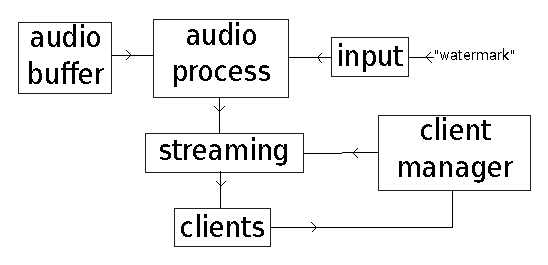
\includegraphics{drawing.eps}
  \caption{The system illustrated by a diagram}

\end{figure}

Seeing how complex the idea of concurrency is, we shift to finding a mechanism to realize this without implement it ourselves. Apparently, it is best that we apply the assistance from a specialized programing language. Partly, to accomplish our original idea, system designing is put at the highest priority, but it would be so much easier if we utilize on a programming language and its intrinsic properties that help us implement this more effectively. After much discussion, we bring another result of our research engineering process into the project as we choose Golang as the programming language for the server application. Golang is a relatively new programming language invented by Google with focus on concurrency. Golang features built-in properties that support concurrency. As mentioned earlier, we modularize our system into smaller parts that work independently. At this point, we apply the goroutine concept from golang to help achieve this. Goroutines are lightweight threads allocated for an instance of a function to execute independently. In our case, we have 4 goroutines that continually running. Golang also introduces channel, as a mean for goroutines to signal each other. For instance, if the input goroutine receive an actual input, it sends the input data through the channel that connects to the audio processing goroutine. Consequently, this function changes its way of processing audio data, switching to do audio embedding with the input data received. Otherwise, the audio processing module would only extract audio data, no watermarking is involed. The streaming goroutine does not care how the audio process deals with data, it only takes audio data that the audio module sends through a channel, and stream to clients. Meanwhile, if there are any new client connect to the streaming point, the client manager goroutine persist the connection for further data streaming. All of those goroutines works independently and signal each other for data. We call this share memory by communicating, not communicate by sharing memory. This is the main compass of the Golang programming language.

With the strong support from Golang, it becomes less painful when implementing the design architecture. However, what Golang does is simply provide us a tool to better systemizing. It is important that we have a solid ground of system design that Golang can relies on and do what it is best at. At the front line, we have the audio processing sequentially scans through the audio file and extract a frame of audio samples with fixed length. This frame is pushed into the queue waiting to be sent to the steaming module, where we also have a queue. The reason why we apply queues to handle data is congestion preventation while also assure a decent amount of spare space for unusually long watermarking information. Specifically, when a big input is received and the current audio frame is not enough for embedding, we should not wait for the next frame because it would increase the overhead cost for the system. What best is take the remaining frames in the queue and fill them up with embedding information. On the other hand, the streaming module also needs a queue to make sure the situation of data starve will not occur. Otherwise, without a queue, if the audio embedding takes too much time to complete, the client have to wait for data to produce sound to listeners, and that is not good at all. 

\section{Experiment}
 
Parameter settings. Our system depends on many parameters in the process of watermark embedding. As we mentioned earlier, it is difficult to achieve an ideal settings when we have many dimensions. For instance, keeping the error rate low enough to not produce an incomplete watermarking, or else it would affect greatly on the user experience. At the same time, we also have to maintain a reasonable amount of embedding space to satisfy the embedding need. Those two are the biggest trade-offs of our system. It then becomes very important to experiement with different settings to come up with a optimal solution for our specific problem. There are two parameter that we need to keep eyes on. First, as we employ the teachnique of dynamic phase coding, we depend on the magnitude of frequency coponents to determine the appropriate phase change. Specifically, we divide our frequency range into \(5\) small part, each with its own setting called step sizes. This number step size is very important to embedd into the phase component of the frequency. If we apply too much shift into the phase components, the audio quaility would decrease. Otherwise, too subtle change could not be successfully decoded. To figure out the best settings, we have to set up several experiments with different ranges of step sizes and record the resulting audio quality as well as the correctness percentage.

In the process of transforming audio data in time domain to the frequency domain, we can choose the range to apply the transformation. At this stage, we can either transform the whole audio file at once or split into smaller frames with fixed length. If we put the whole file into Fourier Transform at once, the frequencies along the files would be mixed together, produce an array of frequencies components from small to big frequency. Numerous components with the same frequencies would be merge into one as our transformation result. Clearly, this approach does not efficient in terms of computation and physics. On one hand, it adds memory overhead as we need to store the enormous transformation result the whole time, while we only need to store a much smaller amount if we split the file into frames. Moreover, mixing frequencies components into only \(1\) component and apply modification would result in the change in all the frequencies components corresponding to that frequency, and of couse this would harm both our audio quality and embedding correctness. Hence, we chose the second approach, spliting audio data into frames with fixed length. However, this result leads us to another question that, what is the resonable length for a frame? 
According to the Nyquist-Shannon sampling theorem, which states that, for a given sample rate \(f_s\), perfect reconstruction is guaranteed possible for a bandlimit \(B<\frac{f_s}{2}\). Plus, recall that the common maximum frequency that human ear can percept is approximately \(20kHz\). Which means, to effectively sample our audio data, we should choose the sample rate \(f_s>40kHz\). It is common in the field of audio processing that we choose \(f_s=44100Hz\) and frame length \(FL=\frac{f_s}{2}=22050\). 

In order to decrease the possibility of embedding into unstable frequencies components, which usually located at frequencies higher than \(1600Hz\). In fact, most of the sound content lies on the low frequency region. Besides, from the property of discrete Fourier transform, the bin corresponding to \(1600Hz\) frequency is at the \(\frac{FL}{f_s}1600=800^{th}\) bin. Hence, we only have \(800\) bins to do embedding.
Next, we look closer into the \(800\) bins we got. To further increase our correctness, we repeat each bit consecutively many times. In particular, we chose \(BITREPEAT=5\), if we have \(1\) bit is incorrectly decoded, we still have \(4\) other bits to rely on. This greatly increase our embedding correctness. As we chose \(BITREPEAT=5\), we only have \(\frac{800}{5}=160\) bits left. But \(8\) bits form a character, which left us \(20\) characters per frame. In summary, we have the following parameters

Evaluation metrics

Experiment results and explanation of the results
\section{Discussion}

How our system is extended/improved to be pratical. This paper provides a glimpse on the massive system. In practice, 

\section{Conclusion}

Summarize our proposed system and its performance

% conference papers do not normally have an appendix


% use section* for acknowledgment
% \section*{Acknowledgment}


% The authors would like to thank...





% trigger a \newpage just before the given reference
% number - used to balance the columns on the last page
% adjust value as needed - may need to be readjusted if
% the document is modified later
%\IEEEtriggeratref{8}
% The "triggered" command can be changed if desired:
%\IEEEtriggercmd{\enlargethispage{-5in}}

% references section

% can use a bibliography generated by BibTeX as a .bbl file
% BibTeX documentation can be easily obtained at:
% http://mirror.ctan.org/biblio/bibtex/contrib/doc/
% The IEEEtran BibTeX style support page is at:
% http://www.michaelshell.org/tex/ieeetran/bibtex/
%\bibliographystyle{IEEEtran}
% argument is your BibTeX string definitions and bibliography database(s)
%\bibliography{IEEEabrv,../bib/paper}
%
% <OR> manually copy in the resultant .bbl file
% set second argument of \begin to the number of references
% (used to reserve space for the reference number labels box)
%\begin{thebibliography}{1}


%\end{thebibliography}




% that's all folks
\end{document}


